\documentclass[conference]{IEEEtran}
\IEEEoverridecommandlockouts

\usepackage{amsmath,amssymb,amsfonts}
\usepackage{booktabs}
\usepackage{graphicx}
\usepackage{cite}
\usepackage{url}
\usepackage{balance}
\usepackage{tikz}
\usepackage{pgfplots}
\usetikzlibrary{arrows.meta,positioning,calc}
\pgfplotsset{compat=1.18}

\newcommand{\BSC}{\mathrm{BSC}_{6}}
\newcommand{\R}{\mathbb{R}}
\newcommand{\Ind}{\mathbf{1}}

\title{Binned Spiking Reservoir Encoding for Perturbation-Characterized Affective ERP Signal Analysis}

\author{
\IEEEauthorblockN{Andrew A. Lane\IEEEauthorrefmark{1}, Wendy Tang\IEEEauthorrefmark{1}, and Brady D. Nelson\IEEEauthorrefmark{2}}
\IEEEauthorblockA{\IEEEauthorrefmark{1}Department of Electrical and Computer Engineering, Stony Brook University, Stony Brook, NY, USA}
\IEEEauthorblockA{\IEEEauthorrefmark{2}Department of Psychology, Stony Brook University, Stony Brook, NY, USA}
}

\begin{document}
\maketitle

\begin{abstract}
Event-related potentials (ERPs) provide high-temporal-resolution measurements of neural response dynamics, but their use in biomedical data analysis is limited by subject variability, low signal-to-noise ratio, and sensitivity to acquisition and preprocessing perturbations. This paper evaluates a fixed spiking reservoir as a nonlinear temporal encoding operator for affective ERP observations. Multichannel ERP traces are transformed by a leaky integrate-and-fire reservoir, summarized using six post-onset spike-count bins, and compressed into a subject-level representation for affective condition analysis. The study tests whether this binned spiking code provides a stable temporal representation under controlled perturbations, rather than claiming classifier superiority over conventional ERP features. Evaluation uses subject-grouped validation, balanced accuracy, macro-F1, classical ERP baselines, and perturbation tests involving additive amplitude noise, temporal jitter, and channel dropout. Results indicate that the reservoir embedding is not a uniformly stronger static classifier than classical ERP-derived features, but it exhibits a distinct perturbation-response profile. The findings support a bounded interpretation of spiking reservoirs as perturbation-characterized temporal measurement operators for biomedical ERP signal analysis.
\end{abstract}

\begin{IEEEkeywords}
EEG, event-related potentials, spiking neural networks, reservoir computing, biomedical signal processing, affective computing, perturbation analysis.
\end{IEEEkeywords}

\section{Introduction}
Electroencephalographic event-related potentials (ERPs) are time-locked measurements of neural response dynamics. In biomedical data analysis, they offer millisecond-scale temporal information but are difficult to model because the observed waveform is a noisy, low-dimensional projection of an unobserved biological dynamical system. Inter-subject variability, trial averaging, volume conduction, and measurement noise can cause endpoint classifiers to conflate temporal structure with subject-specific nuisance variation.

Spiking reservoirs provide one way to construct temporally structured representations without replacing signal analysis by opaque endpoint classification. A fixed recurrent reservoir can act as a nonlinear temporal expansion of the input signal, while spike-count summaries provide discrete observables traceable to post-stimulus time windows. The central question is not whether a spiking reservoir universally outperforms classical ERP features, but which temporal information it preserves, transforms, or suppresses under perturbation.

This paper studies a binned spiking reservoir encoding for affective ERP signal analysis. Each ERP observation is mapped through a fixed leaky integrate-and-fire (LIF) reservoir, summarized by six post-onset spike-count bins, and compressed into a reservoir embedding. Fig.~\ref{fig:pipeline} summarizes the pipeline. The contribution is threefold: (i) formulation of affective ERP analysis as reservoir temporal encoding; (ii) subject-level comparison against classical ERP-derived features using balanced accuracy and macro-F1; and (iii) characterization of the encoding under amplitude noise, temporal jitter, and channel dropout.

\begin{figure}[t]
\centering
\resizebox{\linewidth}{!}{% Figure source: reservoir temporal-encoding pipeline for BIBM 2026.
% Compile through main_bibm2026.tex with TikZ loaded.
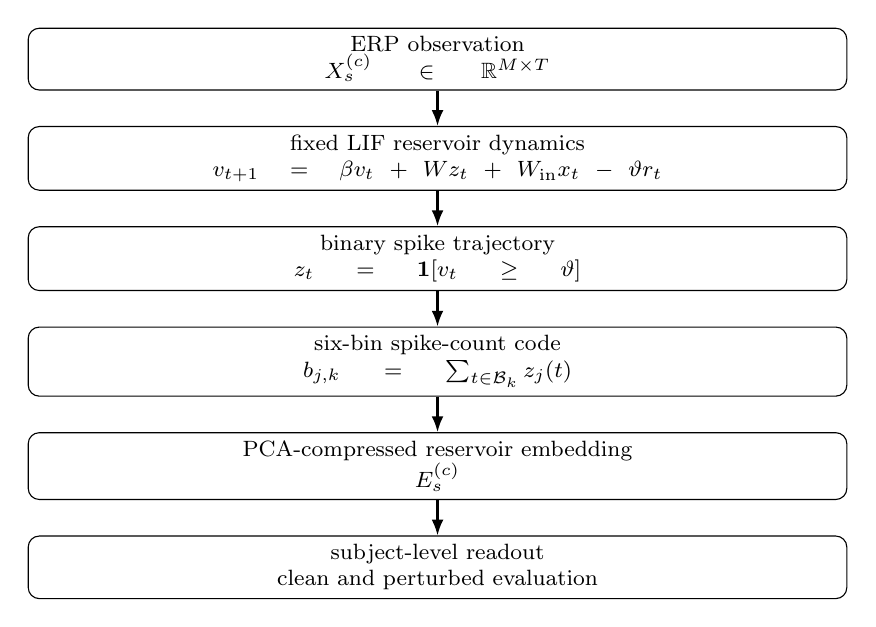
\begin{tikzpicture}[
    font=\footnotesize,
    >=Latex,
    block/.style={draw, rounded corners, align=center, minimum height=7mm, text width=0.84\linewidth, inner sep=3pt},
    arrow/.style={-{Latex[length=2mm]}, thick}
]
\node[block] (x) {ERP observation\\$X_s^{(c)}\in\mathbb{R}^{M\times T}$};
\node[block, below=4.5mm of x] (lif) {fixed LIF reservoir dynamics\\$v_{t+1}=\beta v_t+Wz_t+W_{\mathrm{in}}x_t-\vartheta r_t$};
\node[block, below=4.5mm of lif] (spikes) {binary spike trajectory\\$z_t=\mathbf{1}[v_t\geq\vartheta]$};
\node[block, below=4.5mm of spikes] (bins) {six-bin spike-count code\\$b_{j,k}=\sum_{t\in\mathcal{B}_k}z_j(t)$};
\node[block, below=4.5mm of bins] (embed) {PCA-compressed reservoir embedding\\$E_s^{(c)}$};
\node[block, below=4.5mm of embed] (eval) {subject-level readout\\clean and perturbed evaluation};

\draw[arrow] (x) -- (lif);
\draw[arrow] (lif) -- (spikes);
\draw[arrow] (spikes) -- (bins);
\draw[arrow] (bins) -- (embed);
\draw[arrow] (embed) -- (eval);
\end{tikzpicture}
}
\caption{Reservoir temporal-encoding pipeline. The object of study is the binned spike-count representation induced by fixed LIF reservoir dynamics, not an end-to-end clinical decision model.}
\label{fig:pipeline}
\end{figure}

\section{Methods}
\subsection{ERP Observation Model}
Let $X_s^{(c)}\in\R^{M\times T}$ denote the trial-averaged ERP observation for subject $s$ and affective condition $c$, with $M$ electrodes and $T$ temporal samples. We treat $X_s^{(c)}$ as a noisy observation of an unobserved neural state trajectory:
\begin{equation}
    \xi_{t+1}=f_\theta(\xi_t,u_t)+\eta_t,\qquad x_t=H\xi_t+\epsilon_t,
\end{equation}
where $\xi_t$ is the latent neural state, $H$ is a scalp measurement operator, and $\epsilon_t$ captures measurement and preprocessing noise. This formulation motivates temporal encoders that preserve dynamical information rather than treating the ERP as an unordered feature vector.

\subsection{Spiking Reservoir and Binned Spike Counts}
For each electrode trace, the signal is passed through a fixed LIF reservoir with recurrent weights $W$, input weights $W_{\mathrm{in}}$, leak parameter $\beta$, and firing threshold $\vartheta$:
\begin{align}
    v_{t+1} &= \beta v_t + W z_t + W_{\mathrm{in}}x_t - \vartheta r_t, \\
    z_{t+1} &= \Ind[v_{t+1}\geq \vartheta].
\end{align}
The reservoir is fixed during feature extraction; only the downstream readout is trained.

Post-onset activity is summarized by six equal temporal bins. For reservoir unit $j$ and bin $k$,
\begin{equation}
    b_{j,k}=\sum_{t\in\mathcal{B}_k} z_j(t),\qquad k=1,\ldots,6.
\end{equation}
Fig.~\ref{fig:bsc6} illustrates the temporal-bin observable. Per-electrode spike-bin features are compressed using principal component analysis, and the electrode-level embeddings are concatenated into a trial-level reservoir representation $E_s^{(c)}$.

\begin{figure}[t]
\centering
\resizebox{\linewidth}{!}{% Figure source: BSC6 temporal-bin schematic for BIBM 2026.
% The waveform is schematic; it illustrates binning, not a subject-specific ERP trace.
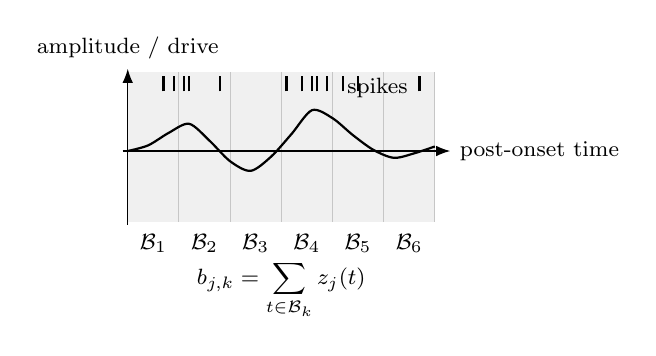
\begin{tikzpicture}[font=\footnotesize, >=Latex]
\begin{scope}[xscale=0.065, yscale=0.72]
    % Six equal post-onset bins.
    \foreach \x/\lab in {0/$\mathcal{B}_1$,10/$\mathcal{B}_2$,20/$\mathcal{B}_3$,30/$\mathcal{B}_4$,40/$\mathcal{B}_5$,50/$\mathcal{B}_6$}{
        \fill[gray!12] (\x,-1.25) rectangle +(10,2.65);
        \draw[gray!45] (\x,-1.25) -- (\x,1.40);
        \node[anchor=north] at (\x+5,-1.30) {\lab};
    }
    \draw[gray!45] (60,-1.25) -- (60,1.40);
    % Axes.
    \draw[-{Latex[length=1.8mm]}] (-1,0) -- (63,0) node[right] {post-onset time};
    \draw[-{Latex[length=1.8mm]}] (0,-1.30) -- (0,1.45) node[above] {amplitude / drive};
    % Schematic ERP / reservoir drive curve.
    \draw[thick, smooth] plot coordinates {
        (0,0.00) (4,0.10) (8,0.32) (12,0.48) (16,0.18)
        (20,-0.18) (24,-0.35) (28,-0.10) (32,0.30) (36,0.72)
        (40,0.58) (44,0.28) (48,0.02) (52,-0.12) (56,-0.04) (60,0.08)
    };
    % Example spikes.
    \foreach \x in {7,9,11,12,18,31,34,36,37,39,42,45,57}{
        \draw[thick] (\x,1.05) -- (\x,1.32);
    }
    \node[anchor=west] at (41,1.12) {spikes};
    \node[align=center, anchor=north] at (30,-1.78) {$\displaystyle b_{j,k}=\sum_{t\in\mathcal{B}_k} z_j(t)$};
\end{scope}
\end{tikzpicture}
}
\caption{Schematic definition of the six-bin spike-count code. Each component $b_{j,k}$ counts spikes from reservoir unit $j$ in post-onset bin $\mathcal{B}_k$, giving the representation temporal traceability at the bin level.}
\label{fig:bsc6}
\end{figure}

\subsection{Baselines, Validation, and Perturbations}
Classical ERP-derived baselines are included to prevent the reservoir from being evaluated against weak comparators. All classifier evaluations use subject-level partitioning: observations from the same subject do not appear simultaneously in training and test folds. Reported metrics include balanced accuracy (BA) and macro-F1.

Two perturbation regimes are separated. Representation-level perturbations corrupt the extracted feature representation and test sensitivity to feature-space amplitude noise and dropout. Raw-signal recomputation applies perturbations before feature extraction and recomputes the reservoir representation. The second regime is stricter because corruption propagates through reservoir dynamics before classification.

\section{Experimental Protocol}
The experiments use a trial-averaged affective ERP dataset with 211 subjects after exclusion of one anomalous subject record. Each subject contributes three affective conditions: negative, neutral, and pleasant, yielding 633 subject-condition observations. The ERP traces contain 34 scalp channels sampled at high temporal resolution and baseline-corrected relative to stimulus onset. The primary task is three-class affective condition analysis. This task is not interpreted as a diagnostic decision problem; it is used as an external label structure for evaluating temporal representation under subject-level validation.

\section{Results}
\subsection{Clean Subject-Level Classification}
Table~\ref{tab:clean} reports clean three-class affective condition performance. The reservoir embedding does not dominate the classical baseline under clean static classification. This constrains the interpretation: the reservoir acts as a nonlinear temporal measurement operator, not as an automatically superior classifier.

\begin{table}[t]
\caption{Clean subject-level affective condition performance.}
\label{tab:clean}
\centering
\begin{tabular}{lccc}
\toprule
Configuration & Feature family & BA & Macro-F1 \\
\midrule
A0 & Classical bandpower/ERP & 0.485 & 0.483 \\
A1 & Reservoir embedding $E$ & 0.463 & 0.460 \\
A2 & Temporal descriptors $D$ & 0.432 & 0.428 \\
A6 & Reservoir + descriptors $E{+}D$ & 0.478 & 0.475 \\
\bottomrule
\end{tabular}
\end{table}

\subsection{Representation-Level Perturbation Response}
Table~\ref{tab:repr_perturb} summarizes representative feature-space perturbation results. Under additive amplitude corruption, the classical bandpower baseline degrades from BA $0.485$ to $0.395$ at 5 dB. The reservoir embedding degrades more weakly, from BA $0.463$ to $0.449$. A similar pattern occurs under feature dropout, where the reservoir embedding remains close to its clean value at 30\% dropout. Fig.~\ref{fig:perturbation} visualizes this contrast.

\begin{table}[t]
\caption{Representation-level perturbation diagnostics.}
\label{tab:repr_perturb}
\centering
\begin{tabular}{llccc}
\toprule
Perturbation & Level & A0 BA & A1 BA & Difference \\
\midrule
Clean & -- & 0.485 & 0.463 & -0.022 \\
Amplitude noise & 5 dB & 0.395 & 0.449 & +0.054 \\
Channel dropout & 30\% & 0.408 & 0.456 & +0.048 \\
\bottomrule
\end{tabular}
\end{table}

\begin{figure}[t]
\centering
% Figure source: representation-level perturbation response for BIBM 2026.
% Values are balanced accuracy from the manuscript tables.
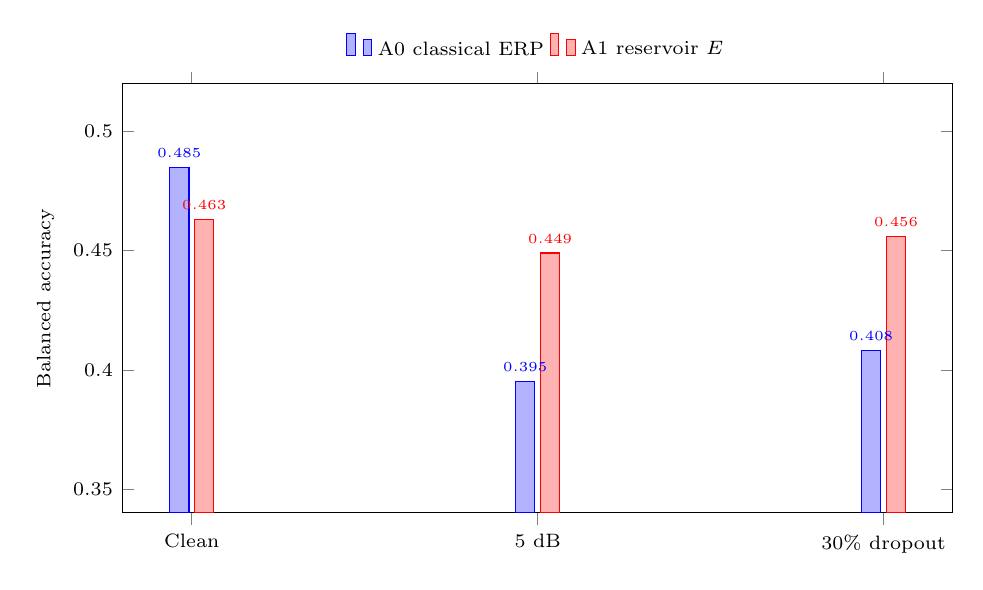
\begin{tikzpicture}
\begin{axis}[
    width=\linewidth,
    height=0.58\linewidth,
    ybar,
    bar width=7pt,
    ymin=0.34,
    ymax=0.52,
    ylabel={Balanced accuracy},
    symbolic x coords={Clean,5 dB,30\% dropout},
    xtick=data,
    x tick label style={font=\scriptsize, align=center},
    y tick label style={font=\scriptsize},
    label style={font=\scriptsize},
    legend style={font=\scriptsize, at={(0.5,1.03)}, anchor=south, legend columns=2, draw=none},
    nodes near coords,
    nodes near coords style={font=\tiny, /pgf/number format/fixed, /pgf/number format/precision=3},
    every axis plot/.append style={draw=black}
]
\addplot coordinates {(Clean,0.485) (5 dB,0.395) (30\% dropout,0.408)};
\addplot coordinates {(Clean,0.463) (5 dB,0.449) (30\% dropout,0.456)};
\legend{A0 classical ERP, A1 reservoir $E$}
\end{axis}
\end{tikzpicture}

\caption{Representation-level perturbation response for the classical ERP baseline (A0) and reservoir embedding (A1). The reservoir embedding has lower clean BA but retains BA more strongly under severe feature-space noise and dropout in this diagnostic regime.}
\label{fig:perturbation}
\end{figure}

\subsection{Raw-Signal Recomputed Perturbations}
A stricter test corrupts the signal before feature extraction and recomputes the representation. Table~\ref{tab:raw_perturb} reports a representative recomputation diagnostic. In this setting, temporal jitter and channel dropout produce larger degradation than the representation-level diagnostic because the perturbations alter the reservoir input trajectory before spike counts are formed.

\begin{table}[t]
\caption{Raw-signal recomputation perturbation diagnostic.}
\label{tab:raw_perturb}
\centering
\begin{tabular}{lcc}
\toprule
Condition & BA & Macro-F1 \\
\midrule
Clean recomputation subset & 0.433 & 0.415 \\
Temporal jitter, $\pm 50$ ms & 0.389 & 0.343 \\
Amplitude noise, 5 dB & 0.429 & 0.408 \\
Channel dropout, 30\% & 0.362 & 0.312 \\
\bottomrule
\end{tabular}
\end{table}

\section{Discussion}
The results support a bounded interpretation of binned spiking reservoirs for affective ERP signal analysis. Under clean static classification, conventional ERP-derived features remain competitive. Under representation-level perturbations, however, the reservoir embedding exhibits a distinct degradation profile, retaining balanced accuracy more strongly than the classical baseline under severe additive noise and dropout. Under raw-signal recomputation, the same embedding remains sensitive to temporal misalignment and channel loss because these perturbations alter the reservoir input trajectory before spike counts are generated.

A reservoir representation is not validated by a single clean accuracy number. It should be characterized by the information it preserves, the transformations it induces, and the conditions under which its dynamics amplify or suppress task-relevant variation. The \BSC{} representation provides temporal traceability because each component corresponds to a post-onset spike-count interval. The recurrent dynamics are fixed, and the downstream readout operates on an extracted representation rather than learning arbitrary temporal filters from the target labels.

Several limitations remain. The dataset is a single affective ERP cohort; the results require external validation before generalization to other EEG paradigms. The study evaluates software-level representations, not neuromorphic hardware energy or latency. The perturbation tests are controlled operating-regime measurements and are not equivalent to full acquisition artifacts. Finally, the present paper isolates the reservoir embedding and does not evaluate graph topology or structure--function coupling.

\section{Conclusion}
This paper evaluated a binned spiking reservoir representation for affective ERP signal analysis under subject-level validation and controlled perturbation tests. The evidence does not support a broad claim that reservoir embeddings dominate classical ERP features for clean static classification. It does support a narrower claim: the reservoir embedding defines a nonlinear temporal measurement operator with a distinct perturbation-response profile. This characterization provides a reproducible basis for studying when event-driven temporal encodings preserve or suppress discriminative structure in biomedical ERP data.

\balance
\begin{thebibliography}{99}
\bibitem{maass2002real} W. Maass, T. Natschlaeger, and H. Markram, ``Real-time computing without stable states: A new framework for neural computation based on perturbations,'' \emph{Neural Computation}, vol. 14, no. 11, pp. 2531--2560, 2002.
\bibitem{jaeger2004harnessing} H. Jaeger and H. Haas, ``Harnessing nonlinearity: Predicting chaotic systems and saving energy in wireless communication,'' \emph{Science}, vol. 304, no. 5667, pp. 78--80, 2004.
\bibitem{lukosevicius2009reservoir} M. Lukosevicius and H. Jaeger, ``Reservoir computing approaches to recurrent neural network training,'' \emph{Computer Science Review}, vol. 3, no. 3, pp. 127--149, 2009.
\bibitem{roy2019towards} K. Roy, A. Jaiswal, and P. Panda, ``Towards spike-based machine intelligence with neuromorphic computing,'' \emph{Nature}, vol. 575, pp. 607--617, 2019.
\bibitem{lawhern2018eegnet} V. J. Lawhern, A. J. Solon, N. R. Waytowich, S. M. Gordon, C. P. Hung, and B. J. Lance, ``EEGNet: A compact convolutional neural network for EEG-based brain-computer interfaces,'' \emph{Journal of Neural Engineering}, vol. 15, no. 5, 056013, 2018.
\bibitem{craik2019deep} A. Craik, Y. He, and J. L. Contreras-Vidal, ``Deep learning for electroencephalogram classification tasks: A review,'' \emph{Journal of Neural Engineering}, vol. 16, no. 3, 031001, 2019.
\bibitem{makeig2004mining} S. Makeig, M. Westerfield, T.-P. Jung, S. Enghoff, J. Townsend, E. Courchesne, and T. J. Sejnowski, ``Dynamic brain sources of visual evoked responses,'' \emph{Science}, vol. 295, no. 5555, pp. 690--694, 2002.
\bibitem{blankertz2011singletrial} B. Blankertz, S. Lemm, M. Treder, S. Haufe, and K.-R. Mueller, ``Single-trial analysis and classification of ERP components---a tutorial,'' \emph{NeuroImage}, vol. 56, no. 2, pp. 814--825, 2011.
\end{thebibliography}


\end{document}
